
\hformbar

\formdesc{Régulateur Numérique}

\formtitle{Loi de commande }

\underline{régulateur PD numérique}
\vspace{3mm}

$u[k] = u[k] + b_0 \cdot e[k]+ b_1 \cdot e[k-1]$ 

avec :


\hfill $b_0 = Kp\cdot(1+\cfrac{T_d}{T_e})$\hfill et \hfill $b_1 = -Kp \cdot \cfrac{T_d}{T_e}$ \hfill

\vspace{3mm}

\underline{régulateur PI numérique}
\vspace{3mm}

$u[k] = u[k] + b_0 \cdot e[k]+ b_1 \cdot e[k-1]$ 

\hformbar


\formdesc{Échantillonnage}

temps d'échantillonnage, sampling h ou $T_s$ 

\begin{center}
    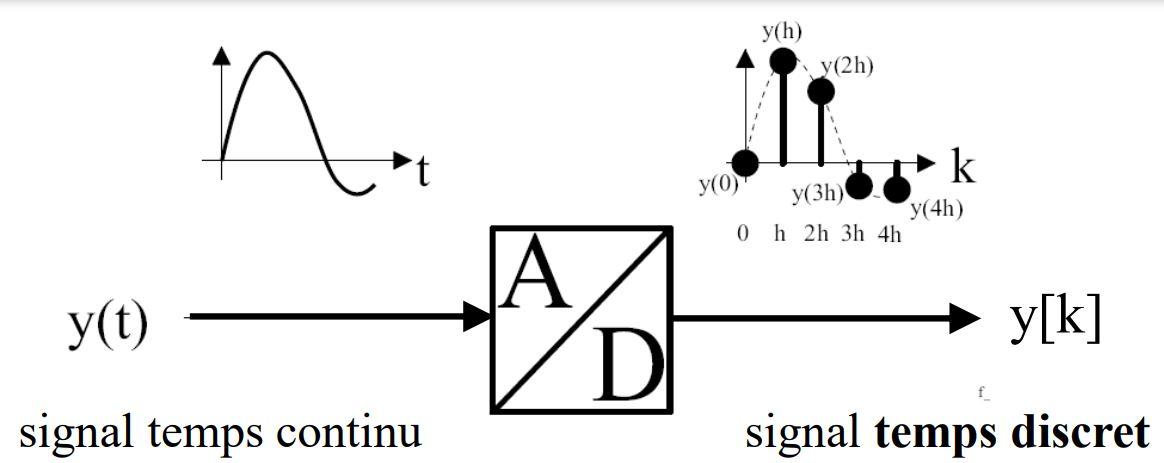
\includegraphics[width = 0.35\textwidth]{img/echantillonage.JPG}
    avec $y[k] = y(k \cdot h)$
\end{center}


Il doit être choisi afin d'éviter les variations trop brutales.

$ h = T_{reg}/20 \; ... \; T_{reg}/10$


\formdesc{Inventaire des retards}

L‘étude « quasi temps-continu » est une première approche pour 
l’analyse et la synthèse approximative d’un système de régulation 
numérique.
Elle est basée sur l’inventaire des retards incontournables que 
possède une boucle de régulation numérique.

Retard du temps de calcul : $T_{cal} < \cfrac{h}{2}$

Retard du bloqueur d'ordre 0 : $T_{rec} \approx \cfrac{h}{2}$

\vspace{3mm}

Retard des conversions :

$T_{convAD} \approx T_{convAD} \approx \cfrac{h}{100} ... \cfrac{h}{10} $


\vspace{2mm}


\vspace{0.5cm}
% Defining string as labels of certain blocks.
\newcommand{\suma}{\Large$+$}
\newcommand{\inte}{$\displaystyle \int$}
\newcommand{\derv}{\huge$\frac{d}{dt}$}

\resizebox{.49\textwidth}{!}{
    \begin{tikzpicture}
        \begin{small} 
            \bXInput{E}
            \bXBloc[4]{algo}{Algo.}{E}
            \bXLink[$w(k)$]{E}{algo}
            \bXBloc[4]{conv1}{D/A}{algo}
            \bXLink[$u(k)$]{algo}{conv1}
            \bXBloc[4]{sys}{Sys.regl.}{conv1}
            \bXLink[$u(t)$]{conv1}{sys}
            \bXOutput[4]{S}{sys}
            \bXLink[$y(t)$]{sys}{S}
            \bXBranchy[4]{S}{U}
            \bXBlocr[12.1]{conv2}{A/D}{U}
            \bXLinkyx{sys-S}{conv2}
            \bXLinkxy[$y(k)$]{conv2}{algo}      
        \node[draw] at (4.8,-2.5) { Retard total : $T_r  =  T_{cal} + T_{convAD} + T_{convAD} + T_{rec} \approx h $};   
        \draw [-latex,red,thick] (3.5,-2.3) to [out=90,in=330] (algo);
        \draw [-latex,blue,thick] (5.3,-2.3) to [out=90,in=320] (conv2);
        \draw [-latex,green!50!black,thick] (6.5,-2.3) to [out=90,in=310] (conv1);
        \draw [-latex,teal!80!purple,thick] (8,-2.3) to [out=90,in=330] (conv1);   
    \end{small}
    \end{tikzpicture}
}



\vspace{3mm}

Ce qui est approximable avec un retard pur par : 

\vspace{3mm}

\underline{Approximations du retard}

\begin{enumerate}
    \item Retard analogique (régime harmonique) :
    
        $e^{-j \omega T_r} = e^{j\varphi}$ avec $\varphi = - \omega T_r$

        $|e^{-j\omega T_r}| = 1$

        $arg(e^{-j\omega T_r}) = -T_r \cdot \omega$

    \item diagramme de Bode du retard analogique exact : 
        \begin{enumerate}
            \item système d'ordre 1 : 
            
                $e^{-j\omega T_r}  \approx \cfrac{1}{1+T_r\cdot j\omega}$

            \item Padé : 
                
                $e^{-j\omega T_r}  \approx \cfrac{1-\cfrac{T_r}{2}j\omega}{1+\cfrac{T_r}{2}j\omega}$

            Exact pour le module (1), mais pas pour la phase !

        \end{enumerate}
\end{enumerate}